
In this sub-chapter, the 1D coil is analysed with an external insulation layer. In the superconducting magnet design community, an assumption is often proposed to simulate the materials behaviour outside of the superconducting cable as a single domain characterised by the properties of G10 which is another material widely used in cryogenics. Such an assumption is made in this thesis. Therefore, both S2-glass as well as D10 are considered to have the material properties of G10.

As it was described at the beginning of the chapter, the longitudinal heat transfer inside the insulation is assumed to be negligible with respect to the transversal one. It is a reasonable assumption because the thermal diffusivity of the strand is several orders of magnitude higher than the one of the insulation layer. It can be proven by calculating the thermal diffusivity ratio between the strand and insulation, as shown in (\ref{eqn: diffusivity_strand_to_insulation_ratio}). As presented in Fig. \ref{fig:diffusivity_strand_to_insulation_ratio}, the thermal diffusivity ratio decreases with rise of temperature but still the insulation thermal diffusivity remains 3 orders of magnitude lower with respect to the strand.

\begin{equation}
    \frac{\alpha_\text{strand}}{\alpha_\text{ins}} = \frac{k_\text{strand}}{k_\text{ins}}~\frac{C_\text{v, ins}}{C_\text{v, strand}}
    \label{eqn: diffusivity_strand_to_insulation_ratio}
\end{equation}

\begin{figure}[h!]
\centering
    \begin{tikzpicture}
        \begin{axis}[
          no markers,
          width=0.7\linewidth, 
          height = 4.5cm,
          xlabel={$T,~\text{K}$},
          ylabel={$\frac{\alpha_{strand}}{\alpha_{ins}}$},
          xmin=0.0,
          ymin=0.0,
          xmax=50.0
          ]
          \addplot table[x=temperature,y=diffusivity_ratio,col sep=comma] {sections/1D_quench_modelling/figures/diffusivity_strand_insul_ratio.csv}; 
        \end{axis}
    \end{tikzpicture}
    \caption{Strand equivalent thermal diffusivity to insulation thermal diffusivity ratio for $B=2~\text{T}$ and $f=2.2$}
    \label{fig:diffusivity_strand_to_insulation_ratio}
\end{figure}



\begin{figure}[h!]
    \centering
    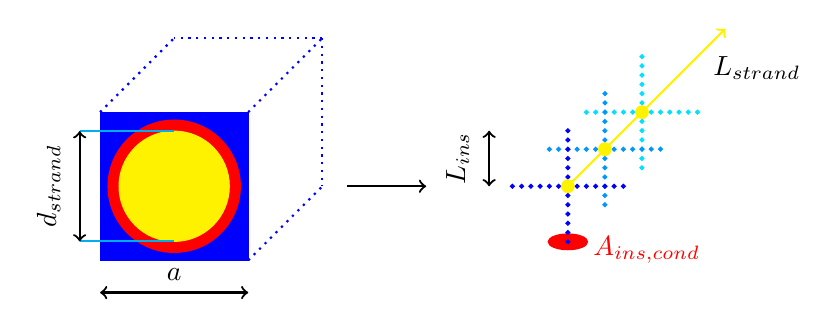
\begin{tikzpicture}[scale = 1]
        \filldraw[blue] (-0.941,-0.941) rectangle (0.941,0.941);
        \filldraw[red] (0,0) circle (0.7+0.07*2);
        \filldraw[yellow] (0,0) circle (0.7);
        \draw[thick, cyan] (-0.8*1.5,0.7) -- (0,0.7);
        \draw[thick, cyan] (-0.8*1.5,-0.7) -- (0,-0.7);
        \draw[black, thick, <->] (-0.75*1.6,0.7) -- (-0.75*1.6,-0.7);
        \node[scale = 1, rotate=90] at (-1.1*1.45, 0) {$d_\text{strand}$};
        \draw[thick,<->] (-0.941,-0.9*1.5) -- (0.941,-0.9*1.5);
        \node[scale = 1] at (0, -0.7*1.6) {$a$};
        \draw[thick, dotted, blue] (0.941,0.941) -- (2*0.941,2*0.941);
        \draw[thick, dotted, blue] (-0.941,0.941) -- (0,2*0.941);
        \draw[thick, dotted, blue] (0.941,-0.941) -- (2*0.941,0);
        \draw[thick, dotted, blue] (2*0.941,2*0.941) -- (2*0.941,0);
        \draw[thick, dotted, blue] (2*0.941,2*0.941) -- (0,2*0.941);
        % ellipse for insulation area
        \filldraw[red] (5.0,-5.646/8) ellipse (0.25cm and 0.1cm);
        \node[scale = 1, red] at (6.0, -5.646/8-0.1) {$A_\text{ins,cond}$};
        % third insulation layer
        \definecolor{blue_third_layer}{RGB}{0,225,255}
        \foreach \x in {-5.646,-4.705,...,5.646} 
            \filldraw[blue_third_layer] (5.0+2*0.4705,\x/8+2*0.4705) circle (0.025);
        \foreach \x in {-5.646,-4.705,...,5.646} 
            \filldraw[blue_third_layer] (5.0+\x/8+2*0.4705,2*0.4705) circle (0.025);
        % second insulation layer
        \definecolor{blue_second_layer}{RGB}{0,150,255}
        \foreach \x in {-5.646,-4.705,...,5.646} 
            \filldraw[blue_second_layer] (5.0+0.4705,\x/8+0.4705) circle (0.025);
        \foreach \x in {-5.646,-4.705,...,5.646} 
            \filldraw[blue_second_layer] (5.0+\x/8+0.4705,0.4705) circle (0.025);
        % first insulation layer
        \definecolor{blue_first_layer}{RGB}{0,0,255}
        \foreach \x in {-5.646,-4.705,...,5.646} 
            \filldraw[blue_first_layer] (5.0,\x/8) circle (0.025);
        \foreach \x in {-5.646,-4.705,...,5.646} 
            \filldraw[blue_first_layer] (5.0+\x/8,0) circle (0.025);
        % strand nodes
        \draw[thick, yellow, ->] (5.0,0) -- (7.0,2.0);
        \foreach \t in {0.0,0.4705,...,1.4115}
            \filldraw[yellow] (5.0+\t,\t) circle (0.08);
        \node[scale = 1] at (7.4, 1.5) {$L_\text{strand}$};    
        \draw[thick, black, <->] (4,0) -- (4,5.646/8);
        \node[scale = 1, rotate=90] at (3.6, 5.646/16) {$L_\text{ins}$}; 
        % draw arrow
        \draw[thick, black, ->] (2.2,0) -- (3.2,0);
    \end{tikzpicture}
    \caption{3-dimensional translation of a 1D+1D strand domain}
    \label{fig: 1d_strand_geometry_with_insulation}
\end{figure}




Insulation dimensions:

\begin{equation}
    A_\text{ins} = a^2 - \frac{\pi d_\text{strand}^2}{4}
\end{equation}

\begin{equation}
    p_\text{avg} = \frac{4 a + \pi d_\text{strand}}{2} 
\end{equation}

\begin{equation}
    L_\text{ins} = \frac{A_\text{ins}}{p_\text{avg}}
\end{equation}

\begin{equation}
    A_\text{ins,cond} = \frac{\frac{1}{4} A_\text{ins} ~ L_{winding}}{L_\text{ins}}
\end{equation}


\begin{figure}[h!]
\centering
    \begin{tikzpicture}
        \begin{axis}[
          no markers,
          width=0.7\linewidth, 
          height = 4.5cm,
          xlabel={$L_\text{strand},~\text{m}$},
          ylabel={$T,~\text{K}$},
          xmin=0.0,
          ymin=0.0,
          xmax=1.0
          ]
        %   Initial temperature curve
          \addplot[smooth, black] table[x=posx,y=t_0_0_ans,col sep=comma] {sections/1D_quench_modelling/figures/results_with_insulation/10ms_1e4elemsf2_2ins_insTem_in.csv};
          
        %   COMSOL plots
          \addplot[smooth, red] table[x=posx,y=t_0_03_com,col sep=comma] {sections/1D_quench_modelling/figures/results_with_insulation/10ms_1e4elemsf2_2ins_insTem_in.csv};
          \addplot[smooth, red] table[x=posx,y=t_0_06_com,col sep=comma] {sections/1D_quench_modelling/figures/results_with_insulation/10ms_1e4elemsf2_2ins_insTem_in.csv};
          \addplot[smooth, red] table[x=posx,y=t_0_1_com,col sep=comma] {sections/1D_quench_modelling/figures/results_with_insulation/10ms_1e4elemsf2_2ins_insTem_in.csv};

        %   ANSYS plots
          \addplot[smooth, blue] table[x=posx,y=t_0_03_ans,col sep=comma] {sections/1D_quench_modelling/figures/results_with_insulation/10ms_1e4elemsf2_2ins_insTem_in.csv};
          \addplot[smooth, blue] table[x=posx,y=t_0_06_ans,col sep=comma] {sections/1D_quench_modelling/figures/results_with_insulation/10ms_1e4elemsf2_2ins_insTem_in.csv};
          \addplot[smooth, blue] table[x=posx,y=t_0_1_ans,col sep=comma] {sections/1D_quench_modelling/figures/results_with_insulation/10ms_1e4elemsf2_2ins_insTem_in.csv};
          
        \end{axis}
    \end{tikzpicture}
    \caption{Temperature distribution calculated in COMSOL (red) and ANSYS (blue) for three time frames: $t=\{0.03, 0.06, 0.1\}$ s.}
    \label{fig: 1d_with_insulation_temp_along_strand_comparison}
\end{figure}

\begin{figure}[h!]
\centering
    \begin{tikzpicture}
        \begin{axis}[
          width=0.7\linewidth, 
          height = 4.5cm,
          xlabel={$L_\text{strand},~\text{m}$},
          ylabel={Relative error, \%},
          xmin=0.0,
          xmax=1.0
          ]
          \addplot[blue, mark=*] table[x=posx,y=error_0_1,col sep=comma] {sections/1D_quench_modelling/figures/results_with_insulation/10ms_1e4elemsf2_2ins_insTem_in_error.csv};
        \end{axis}
    \end{tikzpicture}
    \caption{Relative error along the strand for $t=0.1~\text{s}$.}
    \label{fig: ans_comsol_comparison_f_2_2_with_insulation}
\end{figure}